\documentclass[12px]{scrartcl}

 
\usepackage{float}

\usepackage[utf8]{inputenc}

\usepackage[T1]{fontenc}

\usepackage{lmodern}

\usepackage[ngerman]{babel}

\usepackage{amsmath}

\usepackage{graphicx}


 

\title{Versuch AP2\\ Bestimmung des Planckschen Wirkungsquantums - Der Photoelektrische Effekt}

\author{Frederik Strothmann, Henrik Jürgens}

\date{\today}


\begin{document}


 %deckblatt erstellen

\maketitle
\tableofcontents
\newpage

%einleitung zu dem experiment

\section{Einleitung}

In diesem Versuch wird eine Photozelle (mit Meßverstärker) mit verschiedenen Spektrallinien einer Quecksilberdampflampe beleuchtet, um einen Vergleich zwischen klassischer Theorie und Quantentheorie durchzuführen.
%1
Außerdem wird das Verhältnis $\frac{h}{e}$ und hieraus die Plancksche Konstante h
bestimmt.
%2
In ergänzenden Versuchsteilen können dann umgekehrt aus der Stoppspannung die Wellenlänge des Lichts verschiedenfarbiger Leuchtdioden bestimmt werden.
%3
Außerdem schätzen wir die Quantenausbeute der Photozelle und die Lichtleistung der Quecksilber-Spektrallinien
unter Verwendung einer Halbleiter-Photodiode ab.
%versuchsaufbau mit skizze

\section{Versuchsaufbau}
													
\begin{figure}[H]
\centering
    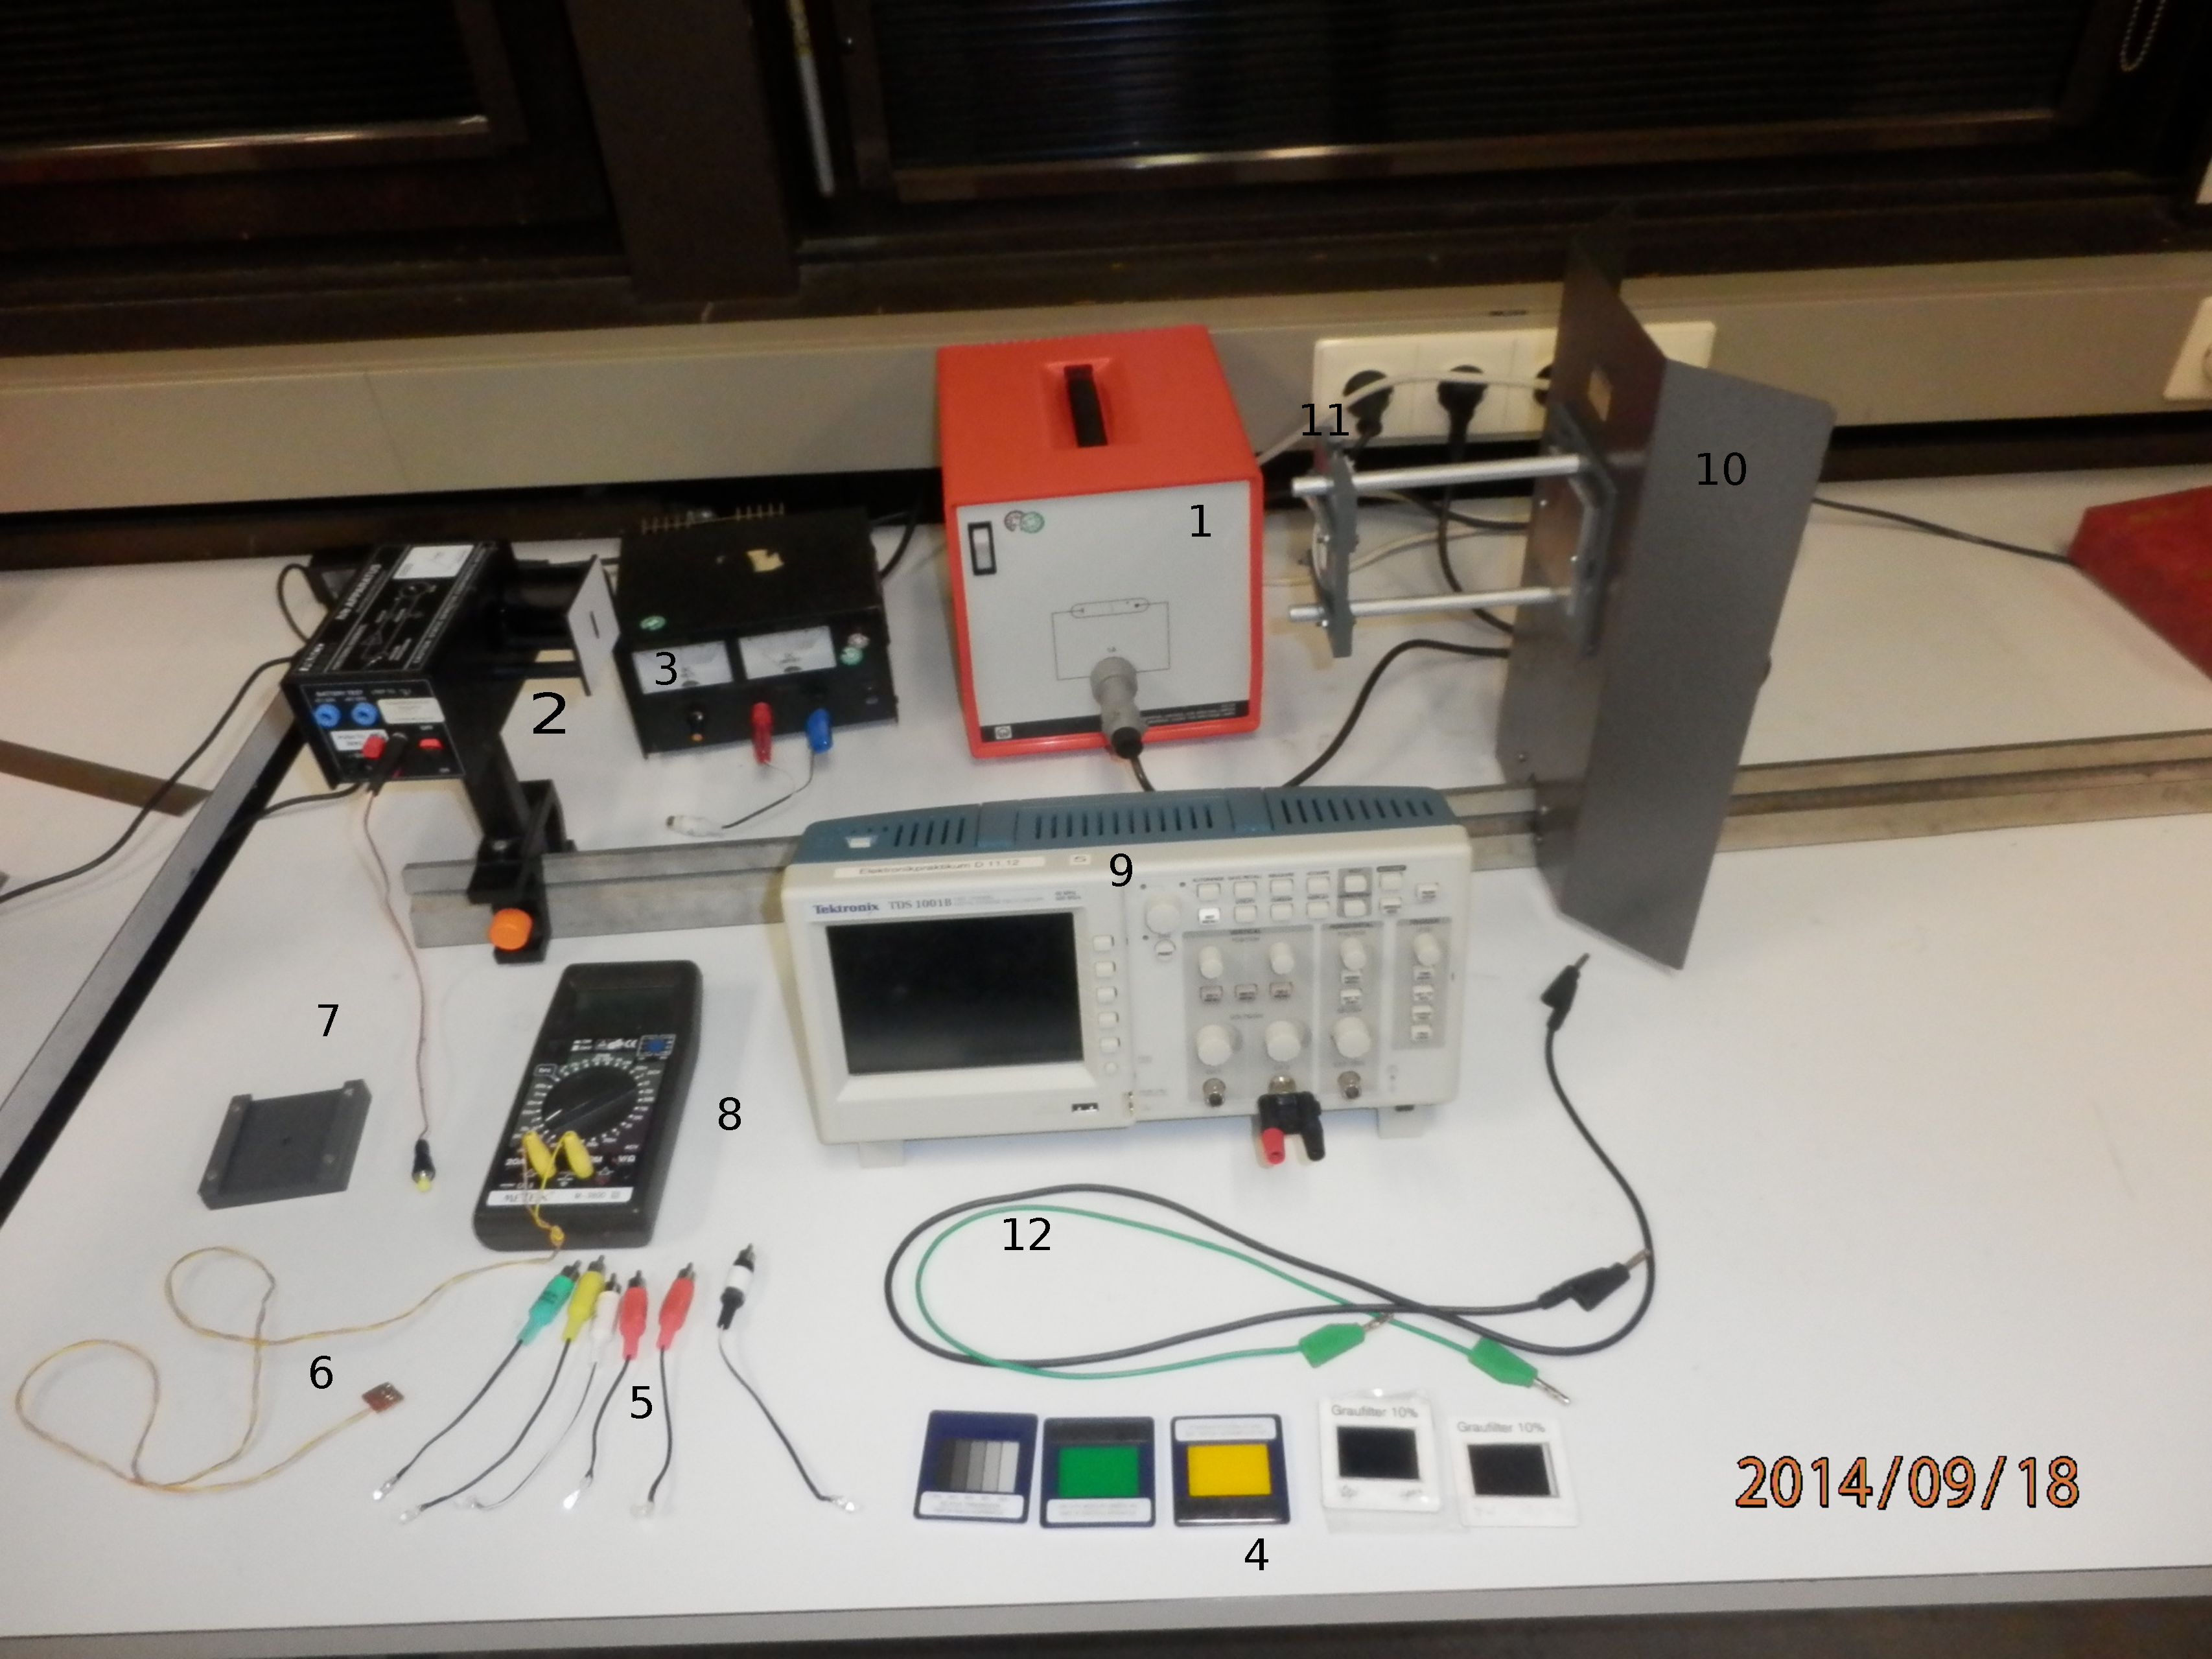
\includegraphics[scale = 0.2]{versuchsmaterialien.pdf}
  	\caption[Für den Versuch verwendete Materialien]{Für den Versuch verwendete Materialien}
  \label{fig:a_3_A}
\end{figure}

\begin{enumerate}
\item	Netzgerät für die Lampe

\item	h/e-Gerät

\item	Netzgerät für die Dioden (5)

\item	grün, gelb, 10\% und 20-100\% Filter

\item	rot, gelb, grün und blaue Dioden

\item	Photodiode

\item	Halterung für die Dioden

\item	DMM

\item	Oszilloskop

\item	Sichtschirm mit dahinter stehender Lampe

\item	Linsengitter Kombination

\item	Verbindungskabel
\end{enumerate}

Das Licht aus der Lampe wird durch die Filterlinsen Kombination in die Spektralfarben aufgespalten, so dass sie mit dem h/e-Gerät die Stopspannung bestimmt werden kann.


\section{Vergleich zwischen Wellen- und Quantenmodell und Bestimmung der Planckschen
Konstante $h$}


\subsection{Praktische Durchführung}
Das Quantenmodell des Lichts besagt, dass die maximale Energie $E_{kin,max}$ von Photoelektronen nur von der Frequenz des einfallenden Lichts abhängt und von der Lichtintensität unabhängig ist.
Dagegen sagt das klassische Wellenmodell des Lichts voraus, dass die maximale Energie $E_{kin,max}$ der Photoelektronen von der Lichtintensität abhängt.
Entsprechend dem Quantenmodell des Lichts ist die Energie der Lichtquanten direkt proportional zu ihrer Frequenz: Je höher die Frequenz, desto mehr Energie hat das Quant. Beim Experimentieren wollen wir den Proportionalitätsfaktor, die Plancksche Konstante, bestimmen.
Wir werden dazu unterschiedliche Spektrallinien der Quecksilberdampflampe verwenden und die Maximalenergie $E_{kin,max}$ der Photoelektronen als Funktion der Wellenlänge und Frequenz untersuchen:
\begin{enumerate}
\item Im (Gitter-)Spektrum der Quecksilberdampflampe sehen wir 5 Farben in mindestens 2 Ordnungen.
%Abbildung 5 aus der versuchsbeschreibung mit den ordnungen einfügen
Wir stellen nun den h/e-Apparat so ein, daß nur eine Farbe aus dem Spektrum erster Ordung (die zweithellste Ordnung) in die Öffnung der Photozelle fällt.
\item Wir messen für jede Farbe der ersten Ordnung die Stoppspannung mit dem Digitalvoltmeter und setzen den
Gelb- bzw. Grünfilter vor den weißen Schirm, falls wir die gelbe bzw. grüne Spektrallinie vermessen.
\item Danach wiederholen wir die Messung für die fünf Farben zweiter Ordnung.
\item Wir benutzen dann die Transmissionsfilter (Graufilter), um die Intensitätsabhängigkeit der Stoppspannung zu messen.
\end{enumerate}
\subsection{Verwendete Formeln}
\textbf{Verwendete Bezeichnungen:}
\begin{enumerate}
\item $U_0$ := Stoppspannung\\ (Kann am $\frac{h}{e}$-Gerät abgelesen werden, da dieses sich wie ein Kondensator verhält, sodass ab einer bestimmten Spannung keine weiteren Elektronen von der Anode aufgenommen werden können.)
\item $h$ := Plancksches Wirkungsquantum\\
(soll in diesem Versuch bestimmt werden)
\item $e$ := Elemetarladung
(Wird in diesem Versuch ohne Fehler angenommen wird, da dieser im Vergleich zu unserer Messung Verschwindend gering ist. $e$= 1,602176...$\cdot10^{-19}C$)
\item $W_0$ := Auslösearbeit\\
(Wird benötigt wird, um die Elektronen von der Materialoberfläche zu lösen)

\end{enumerate}
\textbf{Nach der Einsteinschen Formel ergibt sich für die Stoppspannung die folgende Beziehung:}
\begin{align}
U_0 = \frac{h}{e}\nu + \frac{W_0}{e}
\label{enq:stop}
\end{align}

\subsection{Messergebnisse}
\begin{table}[htbp]
\caption{Frequenz der verschiedenen Farben.}
\begin{center}
\begin{tabular}{|l|r|}
\hline
Farbe & \multicolumn{1}{l|}{Frequenz/GHz} \\ \hline
Ultraviolet & 820264 \\ \hline
Violet  & 740858 \\ \hline
Blau & 687858 \\ \hline
Grün & 548996 \\ \hline
Gelb & 518672 \\ \hline
\end{tabular}
\end{center}
\label{tab:frequenz}
\end{table}



\begin{table}[H]
\caption{Messung der Stoppannung für die 1. Ordnung, der Fehler der Stopspannung wurde mit 0,06V angenommen}
\begin{center}
\begin{tabular}{|l|r|}
\hline
Farbe & \multicolumn{1}{l|}{Spannung/V} \\ \hline
Ultraviolett & 1,58 \\ \hline
Violett & 1,35 \\ \hline
Blau & 1,25 \\ \hline
Grün & 0,71 \\ \hline
Gelb & 0,65 \\ \hline
\end{tabular}
\end{center}
\label{tab:a_1_1}
\end{table}

\begin{table}[H]
\caption{Messung der Stopspannung für die 2. Ordnung, der Fehler der Stopspannung wurde mit 0,06V angenommen}
\begin{center}
\begin{tabular}{|l|r|}
\hline
Farbe & \multicolumn{1}{l|}{Spannung/V} \\ \hline
Ultraviolet & 1,48 \\ \hline
Violet  & 1,25 \\ \hline
Blau & 1,08 \\ \hline
Grün & 0,66 \\ \hline
Gelb & 0,60 \\ \hline
\end{tabular}
\end{center}
\label{tab:a_1_2}
\end{table}

\begin{table}[H]
\caption{Messung der Stopspannung in Abhängigkeit der Intänsität für grünes Licht, der Fehler für die Stopspannung wurde mit 0,06V angenommen}
\begin{center}
\begin{tabular}{|r|r|}
\hline
\multicolumn{1}{|l|}{Filterstärke/\%} & \multicolumn{1}{l|}{Stopspannung/V} \\ \hline
20 & 0,54 \\ \hline
40 & 0,58 \\ \hline
60 & 0,61 \\ \hline
80 & 0,64 \\ \hline
100 & 0,65 \\ \hline
\end{tabular}
\end{center}
\label{tab:intänsität}
\end{table}


\subsection{Auswertung}
%Du musst bei dieser aufgabe beachten, was in der auswertung steht!
In der ersten Aufgabe sollte die Stopspannung in Abhängigkeit der Frequenz graphisch dargestellt werden und nach Gleichung \ref{enq:stop} gefittet werden. Dabei ergab sich für die Messung der 1. Ordnung der folgende Plot (Messwerte aus Tabelle \ref{tab:a_1_1}).

\begin{figure}[H]
\centering
    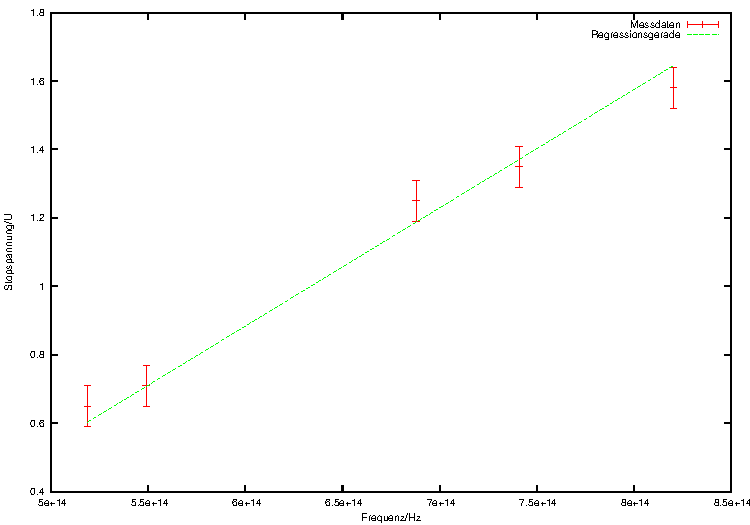
\includegraphics[scale = 1]{a_1_1.pdf}
  	\caption[Plot der Stopspannung, in Abhängigkeit der Frequenz]{Plot der Intensität an Empfänger A, in Abhängigkeit vom Abstand}
  \label{fig:a_3_A}
\end{figure}

Die Regressionsgerade ergab mit f(x)=3,46E-015 $(\pm 2,35E-016) \nu$-1,19 $(\pm 0,1583)$, das reduzierte $\chi^2$ ergab sich mit 1,00175.

Für die 2. Ordnung ergab sich der folgende Plot (Werte aus Tabelle \ref{tab:a_1_2}).

\begin{figure}[H]
\centering
    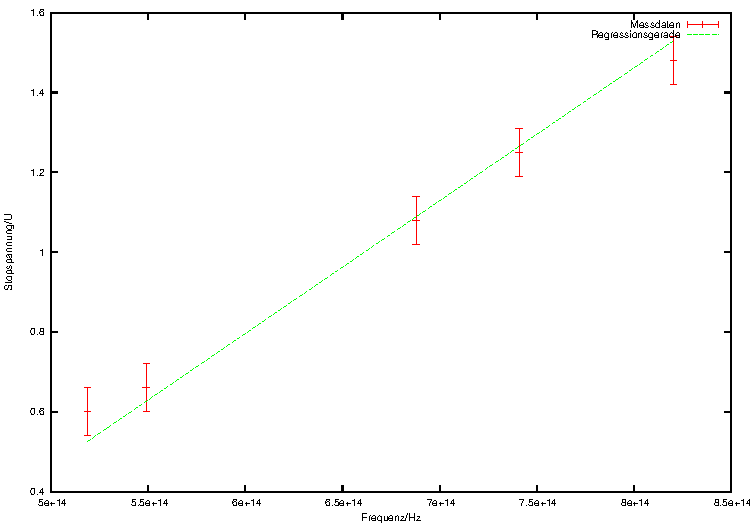
\includegraphics[scale = 1]{a_1_2.pdf}
  	\caption[Plot der Stopspannung, in Abhängigkeit der Frequenz]{Plot der Intensität an Empfänger A, in Abhängigkeit vom Abstand}
  \label{fig:a_3_A}
\end{figure}

Die Regressionsgerade ergab mit f(x)=3,33E-015 $(\pm 2,19E-016) \nu$-1,2 $(\pm 0,1471)$, das reduzierte $\chi^2$ ergab sich mit 0.865638.

Aus der Steigung und dem y-Achsenabschnitt der Regressionsgerade sollten das Plancksche Wirkungsquantum und die Austrittsarbeit bestimmt werden. Für die Messungen der 1. Ordnung wurde das Plancksche Wirkungsquantum mit 5,5E-034 $(\pm 0,4E-034)$ Js und die Austrittsarbeit mit -1,9E-019 $(\pm 0,3E-019)$ J. Für die Messung der 2. Ordnung wurde h mit 5,33E-034 $(\pm 0,35E-034)$ Js und die Austrittsarbeit mit -1,9E-019 $(\pm 0,2E-019)$ bestimmt.

Zum Schluss der Messung wurde noch die Abhängigkeit der Stopspannung von der Intensität dazu wurde ein 20\%, 40\%, 60\%, 80\% und 100\% durchlässiger Intensitätsfilter  verwendet. Die Messdaten finden sich in Tabelle \ref{tab:intänsität}. Die abfallende Stopspannung entsteht offensichtlich durch Leckströme unseres h/e-Geräts (der "Kondensator" entlädt sich schneller, als der Aufladevorgang durch den Photostrom).

\subsection{Diskussion}
Das Plancksche Wirkungsquantum hat einen Literaturwert von 6,6$\cdot 10^34$ Js\footnote{Entnommen von http://de.wikipedia.org/wiki/Plancksches\_Wirkungsquantum am  18.09.2014 um 16:15 Uhr}, unsere Wert für die Messung der 1. Messung weicht um 16,6\% ab. Der Wert aus der Messung der 2. Ordnung weicht um 19,7\% ab. Diese große  Abweichung erklärt sich über die großen Leckströme, wodurch die von uns gemessene Spannung nicht die echte Stopspannung ist und wir eine zu geringe Spannung gemessen haben.

\section{Abschätzung des Photostroms; Quantenausbeute der Photozelle und Lichtleistung}
\subsection{1. Kondensatorkapazität und Photostrom}
\subsubsection{Praktische Durchführung}
Die Photozelle und der Eingang des Meßverstärkers im h/e-Apparat bilden einen kleinen Kondensator, der durch den Photostrom aufgeladen und durch Leckströme im Meßverstärker entladen wird.
Wir wollen aus der Halbwertszeit für den Auf- und Entladevorgang, sowie der Stoppspannung $U_0$ die Kondensatorkapazität und den Photostrom abschätzen. Die Entladekurven haben wir mit einem Oszilloskop vermessen, da unsere Leckströme sehr groß waren.
\subsubsection{Verwendete Formeln}
\textbf{Verwendete Bezeichnungen:}
\begin{enumerate}
\item $I_{ph}$ := Photonenstrom
\item $U_0$ := Stoppspannung
\item $R$ := 'Aufladewiderstand'\\
(Modellhaft wird der Kondensator über einen Widerstand aufgeladen, trivialerweise ergibt sich der verwendete Zusammenhang aus der zugehörigen Differentialgleichung)
\item $t_{1/2_a}$ := Halbwertszeit des Aufladevorgangs
\item $C_{\frac{h}{e}}$ := Kapazität des $\frac{h}{e}$-Gerätes
\item $t_{1/2_e}$ := Halbwertszeit des Entladevorgangs
\item $R_i$ := Innenwiderstand des $\frac{h}{e}$-Gerätes\\
(Der Widerstand charakterisiert die auftretenden Leckströme im $\frac{h}{e}$-Gerät. Er wurde in der Versuchsanleitung mit ca. 10$^{13}\omega$ geschätzt. Da wir sehr große Leckströme hatten und unser Gerät sehr alt ist, ist der Widerstand  mittlerweile warscheinlich viel kleiner. Der daraus errechnete Photostrom gibt deshalb nur die Größenordnung, in der wir uns befinden, an.)
\end{enumerate}
\textbf{Aus den beiden Halbwertszeiten für den Auf- und Entladevorgang und der Stoppspannung bestimmen wir den Photostrom nach der folgenden Formel:}
\begin{align}
I_{ph} = \frac{U_0}{R}
\end{align}
Dazu muss einerseits der 'Aufladewiderstand'
\begin{align}
R = \frac{t_{1/2_a}}{\ln(2)C_{\frac{h}{e}}}
\end{align}
und andererseits die Kapazität unseres $\frac{h}{e}$-Gerätes bestimmt werden.
\begin{align}
C_{\frac{h}{e}} = \frac{t_{1/2_e}}{\ln(2)R_i}
\end{align}
\subsubsection{Messergebnisse}
\subsubsection{Auswertung}
\subsubsection{Diskussion}

\subsection{2. Die Photozelle als Spektrometer}
Es stehen uns verschiedene Leuchtdioden zur Verfügung. Diese schließen wir an ein Netzgerät an.
(Strom etwa 20 mA, wird durch einen Widerstand bzw. Regler im Anschlußstecker begrenzt), Es ist zu beachten, dass Leuchtdioden -- wie gewöhnliche Dioden auch -- nur in einer Stromrichtung arbeiten.
Wir befestigen die Leuchtdioden nacheinander in der 5-mm-Bohrung einer Kunststoffhalterung und schieben die Halterung waagerecht so über den weißen Schirm des h/e-Apparates, dass das Licht auf die Photozelle gelangen kann. Wir bestimmen dann die jeweiligen Stoppspannungen.
Mit den Ergebnissen aus Versuchsteil 1 können wir, durch Messung der Stoppspannung, die Wellenlänge des Lichtes bestimmen. Diese vergleichen wir mit den Wellenlängen, welche in den Datenblättern der Leuchtdioden angegeben sind. (siehe auch Beschriftung an den Leuchtdioden):
rot = 645 nm, gelb = 583 nm, grün = 565 nm, blau = 470 nm.
%Erklären Sie die Abweichungen zum Literaturwert.
\subsubsection{Verwendete Formeln}
\subsubsection{Messergebnisse}
\subsubsection{Auswertung}
\subsubsection{Diskussion}

\subsection{3. Quantenausbeute der Photozelle und Lichtleistung}
Nicht jedes erzeugte Photoelektron gelangt zur Anode, wenn -- wie in unserem Versuchsaufbau -- die
Photozelle ohne hohe Vorspannung betrieben wird. Die Zahl der im Photostrom nachgewiesenen Photoelektronen ist viel kleiner als die Anzahl der einfallenden Lichtquanten. %(warum?)
Wir wollen das Verhältnis zwischen der Anzahl $N_{ph}$ der Photonen (Lichtquanten), die von der Lichtquelle ausgehend in die Photozelle einfallen, zur
Anzahl $N_{e,Zelle}$ der Elektronen, die von diesen Photonen in der Photozelle produziert werden und den Photostrom bewirken, abschätzen, also: Quantenausbeute = $\frac{N_{e,Zelle}} {N_{ph}}$.
Dazu verwenden wir folgendes Verfahren: Für diese Messung steht uns eine Halbleiter-Photodiode zur Verfügung. Eine solche Photodiode besteht aus einem kleinen Halbleiterkristall. Fällt Licht auf die strahlungsempfindliche Fläche (hier 2, 75 $\times$ 2, 75 mm groß), so werden durch den inneren Photoeffekt Ladungsträger erzeugt, es fließt ebenfalls ein Photostrom. In der Photodiode erzeugt fast jedes einfallende Photon ein Elektron: bei einer Wellenlänge von 850 nm werden
etwa 88 Elektronen pro 100 Lichtquanten erzeugt, für andere Wellenlängen ist das Verhältnis geringer.
Die folgende Abbildung zeigt die Abhängigkeit der relativen spektralen Empfindlichkeit für unseren Photodioden-
typ BPW34 (100 \% entsprechen 88 Elektronen pro 100 Quanten).
%bitte abbildung für die relative empfindlichkeit der photodiode einfügen
Wir schließen die Photodiode an ein Digitalmultimeter an, Messbereich 200 $\mu$A. Die Polarität ist nicht wichtig. Wir halten die Photodiode in den Strahlengang, sodass das Licht einer Spektrallinie auf die Photodiode fällt. Es ist zu beachten, dass die Photodiode etwa den gleichen Abstand von der Lichtquelle hat wie die Photozelle.
%(warum?)
Wir Klappen daher das Lichtschutzrohr zur Seite
und halten die Photodiode vor der Photozelle in das Licht der Spektrallinie.
Wir messen den Photostrom für diese und die anderen Spektrallinien.
Wir können jetzt vom Photostrom der Photodiode auf die Zahl der Elektronen und daraus -- je nach Wellenlänge -- auf die Anzahl der Photonen (pro Zeitintervall) schließen. Wir nehmen an, dass die Öffnung an der Photozelle etwa so groß ist wie die Fläche der Photodiode, d.h. beide erhalten etwa gleich viel Photonen — vorausgesetzt, beide haben den gleichen Abstand zur Lichtquelle. Den Photostrom der Photozelle haben wir in Teil 1 abgeschätzt. Hiermit bestimmen wir die Quantenausbeute der Photozelle. Wir haben die Anzahl der Photonen (pro Zeitintervall) bestimmt; aus der Wellenlänge und der Planckschen Konstanten können wir die Energie jedes Photons berechnen. Wir bestimmen wir die Lichtleistung, die mit den einzelnen Spektrallinien auf die Photozelle gelangt.

\subsubsection{Verwendete Formeln}
\subsubsection{Messergebnisse}
\subsubsection{Auswertung}
\subsubsection{Diskussion}

\section{Fazit}

 %Werte stimmen mit den Formeln überein/nicht überein

\end{document}

